\documentclass{memoir}
\usepackage{notestemplate}

\usetikzlibrary{arrows,chains,matrix,positioning,scopes}

\makeatletter
\tikzset{join/.code=\tikzset{after node path={%
\ifx\tikzchainprevious\pgfutil@empty\else(\tikzchainprevious)%
edge[every join]#1(\tikzchaincurrent)\fi}}}
\makeatother

\tikzset{>=stealth',every on chain/.append style={join},
every join/.style={->}}
%\logo{~/School-Work/Auxiliary-Files/resources/png/logo.png}
%\institute{Rice University}
%\faculty{Faculty of Whatever Sciences}
%\department{Department of Mathematics}
%\title{Class Notes}
%\subtitle{Based on MATH xxx}
%\author{\textit{Author}\\Gabriel \textsc{Gress}}
%\supervisor{Linus \textsc{Torvalds}}
%\context{Well, I was bored...}
%\date{\today}

%\makeindex

\begin{document}

% \maketitle

% Notes taken on 

Let \(A\) and \(C\) be arbitrary groups.. One question worth exploring is if there exists a group \(B\) such that \(A / B \cong C\)-- that is, \(B\) is an extension of \(C\) by \(A\). The tools we develop to understand this question are exact sequences. If \(A\) is isomorphic to a subgroup of \(B \), there is an injective homomorphism from \(A\) to \(B\). And if \(C\) is isomorphic to the quotient, then there is a surjective homomorphism from \(B\) to \(C\). This will give us a chain
\begin{align*}
	A \to B \to C
\end{align*}
where the homomorphisms are compatible with. We formalize this idea via exact sequences.

\begin{defn}[Exact Sequences]
	Let \(\alpha ,\beta \) be homomorphisms so that
	\begin{align*}
		X \to^{\alpha } Y \to^{\beta }Z.
	\end{align*}
	If \(\textrm{Im}(\alpha ) = \textrm{Ker}(\beta )\), then we say the pair of homomorphisms are \textbf{exact}.\\

	A sequence of homomorphisms
	\begin{align*}
		\ldots \to X_{n-1} \to X_n \to X_{n+1} \to \ldots
	\end{align*}
	is said to be an \textbf{exact sequence} if it is exact at every \(X_n\) between a pair of homomorphisms.
\end{defn}
Hence, our goal is to see whether we can form an exact sequence \(A\to B\to C\). Our notions of injectivity and surjectivity correspond exactly to the notions of exactness.
\begin{prop}
	Let \(A,B,C\) be groups. Then the sequence
	\begin{align*}
		0 \to A \to^{\psi }B
	\end{align*}
	is exact at \(A\) if and only if \(\psi \) is injective. Likewise, the sequence
	\begin{align*}
		B \to^{\varphi }\to C \to 0
	\end{align*}
	is exact at \(C\) if and only if \(\varphi \) is surjective.
\end{prop}
Combining the two ideas, the sequence
\begin{align*}
	0 \to A \to^{\psi }B \to^{\varphi }C \to 0
\end{align*}
is exact if and only if \(\psi \) is injective, \(\varphi \) is surjective, and \(\textrm{Im}(\psi ) = \textrm{Ker}(\varphi )\).

\begin{defn}
	An exact sequence of the form
	\begin{align*}
		0 \to A \to^{\psi }B \to^{\varphi }C \to 0
	\end{align*}
	is called an \textbf{short exact sequence}.
\end{defn}
Our goal then is to determine if two groups admit a short exact sequence, and if so, how many.\\

Notice that any exact sequence can be written as a succession of short exact sequences. For example, if
\begin{align*}
	X \to^{\alpha }Y \to^{\beta }Z
\end{align*}
is exact at \(Y\), then equivalently
\begin{align*}
	0 \to \alpha (X) \to Y \to Y / \textrm{Ker}(\beta ) \to 0
\end{align*}
is a short exact sequence.

\begin{exmp}
	
\end{exmp}

For fixed \(A,C\), there can be many extensions of \(C\) by  \(A\). Hence, we need to determine a notion of a homomorphism to distinguish exact sequences.

\begin{defn}[Homomorphism of Short Exact Sequences]
	Let
	\begin{align*}
		0 \to A \to B \to C \to 0\\
		0 \to A' \to B' \to C' \to 0
	\end{align*}
	be two short exact sequences of groups. A \textbf{homomorphism of short exact sequences} is a collection of group homomorphisms \(\alpha ,\beta ,\gamma \) such that the following diagram commutes:
\begin{center}
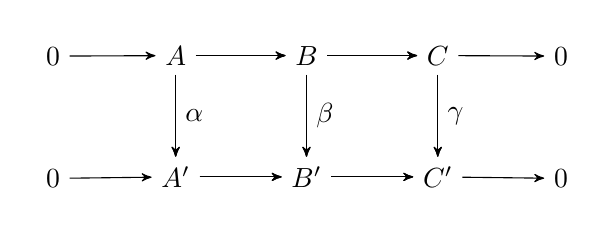
\begin{tikzpicture}
  \matrix (m) [matrix of math nodes, row sep=3em, column sep=3em]
    { 0 & A  & B  & C  & 0 \\
      0 & A' & B' & C' & 0 \\ };
  { [start chain] \chainin (m-1-1);
    \chainin (m-1-2);
    { [start branch=A] \chainin (m-2-2)
        [join={node[right] {$\alpha $}}];}
    \chainin (m-1-3) [join={node[above] {}}];
    { [start branch=B] \chainin (m-2-3)
        [join={node[right] {$\beta $}}];}
    \chainin (m-1-4) [join={node[above] {}}];
    { [start branch=C] \chainin (m-2-4)
        [join={node[right] {$\gamma $}}];}
    \chainin (m-1-5); }
  { [start chain] \chainin (m-2-1);
    \chainin (m-2-2);
    \chainin (m-2-3) [join={node[above] {}}];
    \chainin (m-2-4) [join={node[above] {}}];
    \chainin (m-2-5); }
\end{tikzpicture}
\end{center}
This is an \textbf{isomorphism of short exact sequences} if \(\alpha ,\beta ,\gamma \) are isomorphisms in which case the extensions \(B,B'\) are \textbf{isomorphic extensions}.\\

The two exact sequences are called \textbf{equivalent} if \(A = A'\), \(C = C'\), and there is an isomorphism between them where  \(\alpha ,\gamma \) are identity. In this case \(B\) and \(B'\) are \textbf{equivalent extensions}.
\end{defn}
Equivalency by extensions is strongesomorphisms between \(B\) and \(B'\)-- it tells us that there is an isomorphism between \(B\) and \(B'\) that restricts to an isomorphism from \(A\) to \(A'\) and induces an isomorphism on the quotients by \(C\) and \(C'\).

\begin{exmp}
	
\end{exmp}

\begin{prop}[Short Five Lemma]
	Let \(\alpha ,\beta ,\gamma \) be a homomorphism of short exact sequences
\begin{center}
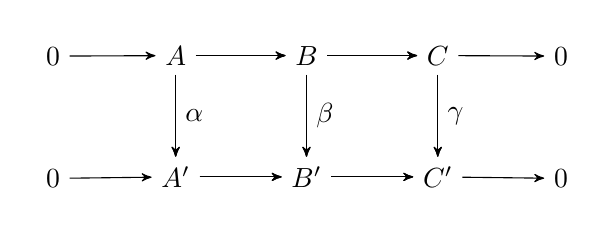
\begin{tikzpicture}
  \matrix (m) [matrix of math nodes, row sep=3em, column sep=3em]
    { 0 & A  & B  & C  & 0 \\
      0 & A' & B' & C' & 0 \\ };
  { [start chain] \chainin (m-1-1);
    \chainin (m-1-2);
    { [start branch=A] \chainin (m-2-2)
        [join={node[right] {$\alpha $}}];}
    \chainin (m-1-3) [join={node[above] {}}];
    { [start branch=B] \chainin (m-2-3)
        [join={node[right] {$\beta $}}];}
    \chainin (m-1-4) [join={node[above] {}}];
    { [start branch=C] \chainin (m-2-4)
        [join={node[right] {$\gamma $}}];}
    \chainin (m-1-5); }
  { [start chain] \chainin (m-2-1);
    \chainin (m-2-2);
    \chainin (m-2-3) [join={node[above] {}}];
    \chainin (m-2-4) [join={node[above] {}}];
    \chainin (m-2-5); }
\end{tikzpicture}
\end{center}
\begin{itemize}
	\item If \(\alpha ,\gamma \) are injective then so is \(\beta \) 
	\item If \(\alpha ,\gamma \) are surjective then so is \(\beta \) 
	\item If \(\alpha ,\gamma \) are isomorphisms then so is \(\beta \)
\end{itemize}
\end{prop}

\begin{proof}[Proof of Short Five Lemma]
	
\end{proof}
There is always at least one extension of a group \(C\) by \(A\) given by \(B = A \rtimes C\).

\begin{defn}
	If
	\begin{align*}
		1 \to A \to^{\psi }B \to^{\varphi }C \to 1
	\end{align*}
	is a short exact sequence of groups, then the sequence is \textbf{split} if there is a sugroup complement to \(\psi (A)\) in \(B\). Then up to isomorphism \(B = A \rtimes C\) up to isomorphism by
	\begin{align*}
		B = \psi (A) \rtimes C'
	\end{align*}
	for some subgroup \(C'\), which satisfies \(\varphi (C') \cong C\).\\

	We say \(B\) is a \textbf{split extension of \(C\) by \(A\)}.
\end{defn}
This is really just the question of existence of a complement to \(\psi (A)\) in \(B\) that is isomorphic by \(\varphi \) to \(C\).

\begin{prop}
	The short exact sequence of groups
	\begin{align*}
		1 \to A \to^{\psi }B \to^{\varphi }C \to 0
	\end{align*}
	of groups is split if and only if there is a group homomorphism \(\mu :C\to B\) such that \(\varphi \circ \mu \cong \textrm{Id}_C \).\\

	Any set map \(\mu :C\to B\) such that \(\varphi \circ \mu = \textrm{Id}_C\) is called a \textbf{section} of \(\varphi \). If \(\mu \) is a homomorphism, then \(\mu \) is called a \textbf{splitting homomorphism} for the sequence.
\end{prop}
A section of \(\varphi \) is merely a choice of coset representative in \(B\) for \(B / \textrm{Ker}\varphi  \cong C\). A section is a splitting homomorphism if this set of coset representatives forms a subgroup, in which case this subgroup gives a complement to \(\psi (A)\) in \(B\).

\begin{exmp}
	
\end{exmp}

\begin{prop}
	Let
	\begin{align*}
		0 \to A \to^{\psi }B \to^{\varphi }C \to 0
	\end{align*}
	be a short exact sequence of groups. Then \(B = \psi (A) \rtimes C'\) for some subgroup \(C'\) of \(B\) with \(\varphi (C') \cong C\) if and only if there is a homomorphism \(\lambda :B\to A\) such that \(\lambda \circ \psi = \textrm{Id}_A\) .
\end{prop}
This is stronger than the previous proposition. The existence of a splitting homomorphism on the left end of the sequence gives that the extension group is a direct product (instead of a semidirect product).

% \printindex
\end{document}
